Partimos de la base que somos una empresa a la que se la ha adjudicado el despliegue de infraestructura de red 4G, con el objetivo de prestar servicio a vehículos conectados. Dicho servicio queremos que se implemente en la autovía que conecta la ciudad de Salamanca con Tordesillas, en Castilla y León. \\

El tramo de carretera seleccionado comprende 73 kilómetros, en concreto desde el kilómetro 158 al kilómetro 231 de la A-62. En dicho tramo nos encontramos con que ya existe una buena infraestructura de red 4G prestando servicio, por ello vamos a aprovechar parte de ella. En concreto, haremos uso de las torres de telefonía ya disponibles, disponemos de 11 a lo largo de la carretera, tal y como podemos observar en la figura \ref{autovia}. En las torres que sean necesarias, que no tienen por qué ser todas, instalaremos nuestros propios equipos, como estaciones base y antenas. Es importante evaluar cuidadosamente los costos asociados a los componentes y considerar opciones con precios competitivos. \\


\begin{figure}[H]
    \centering
 	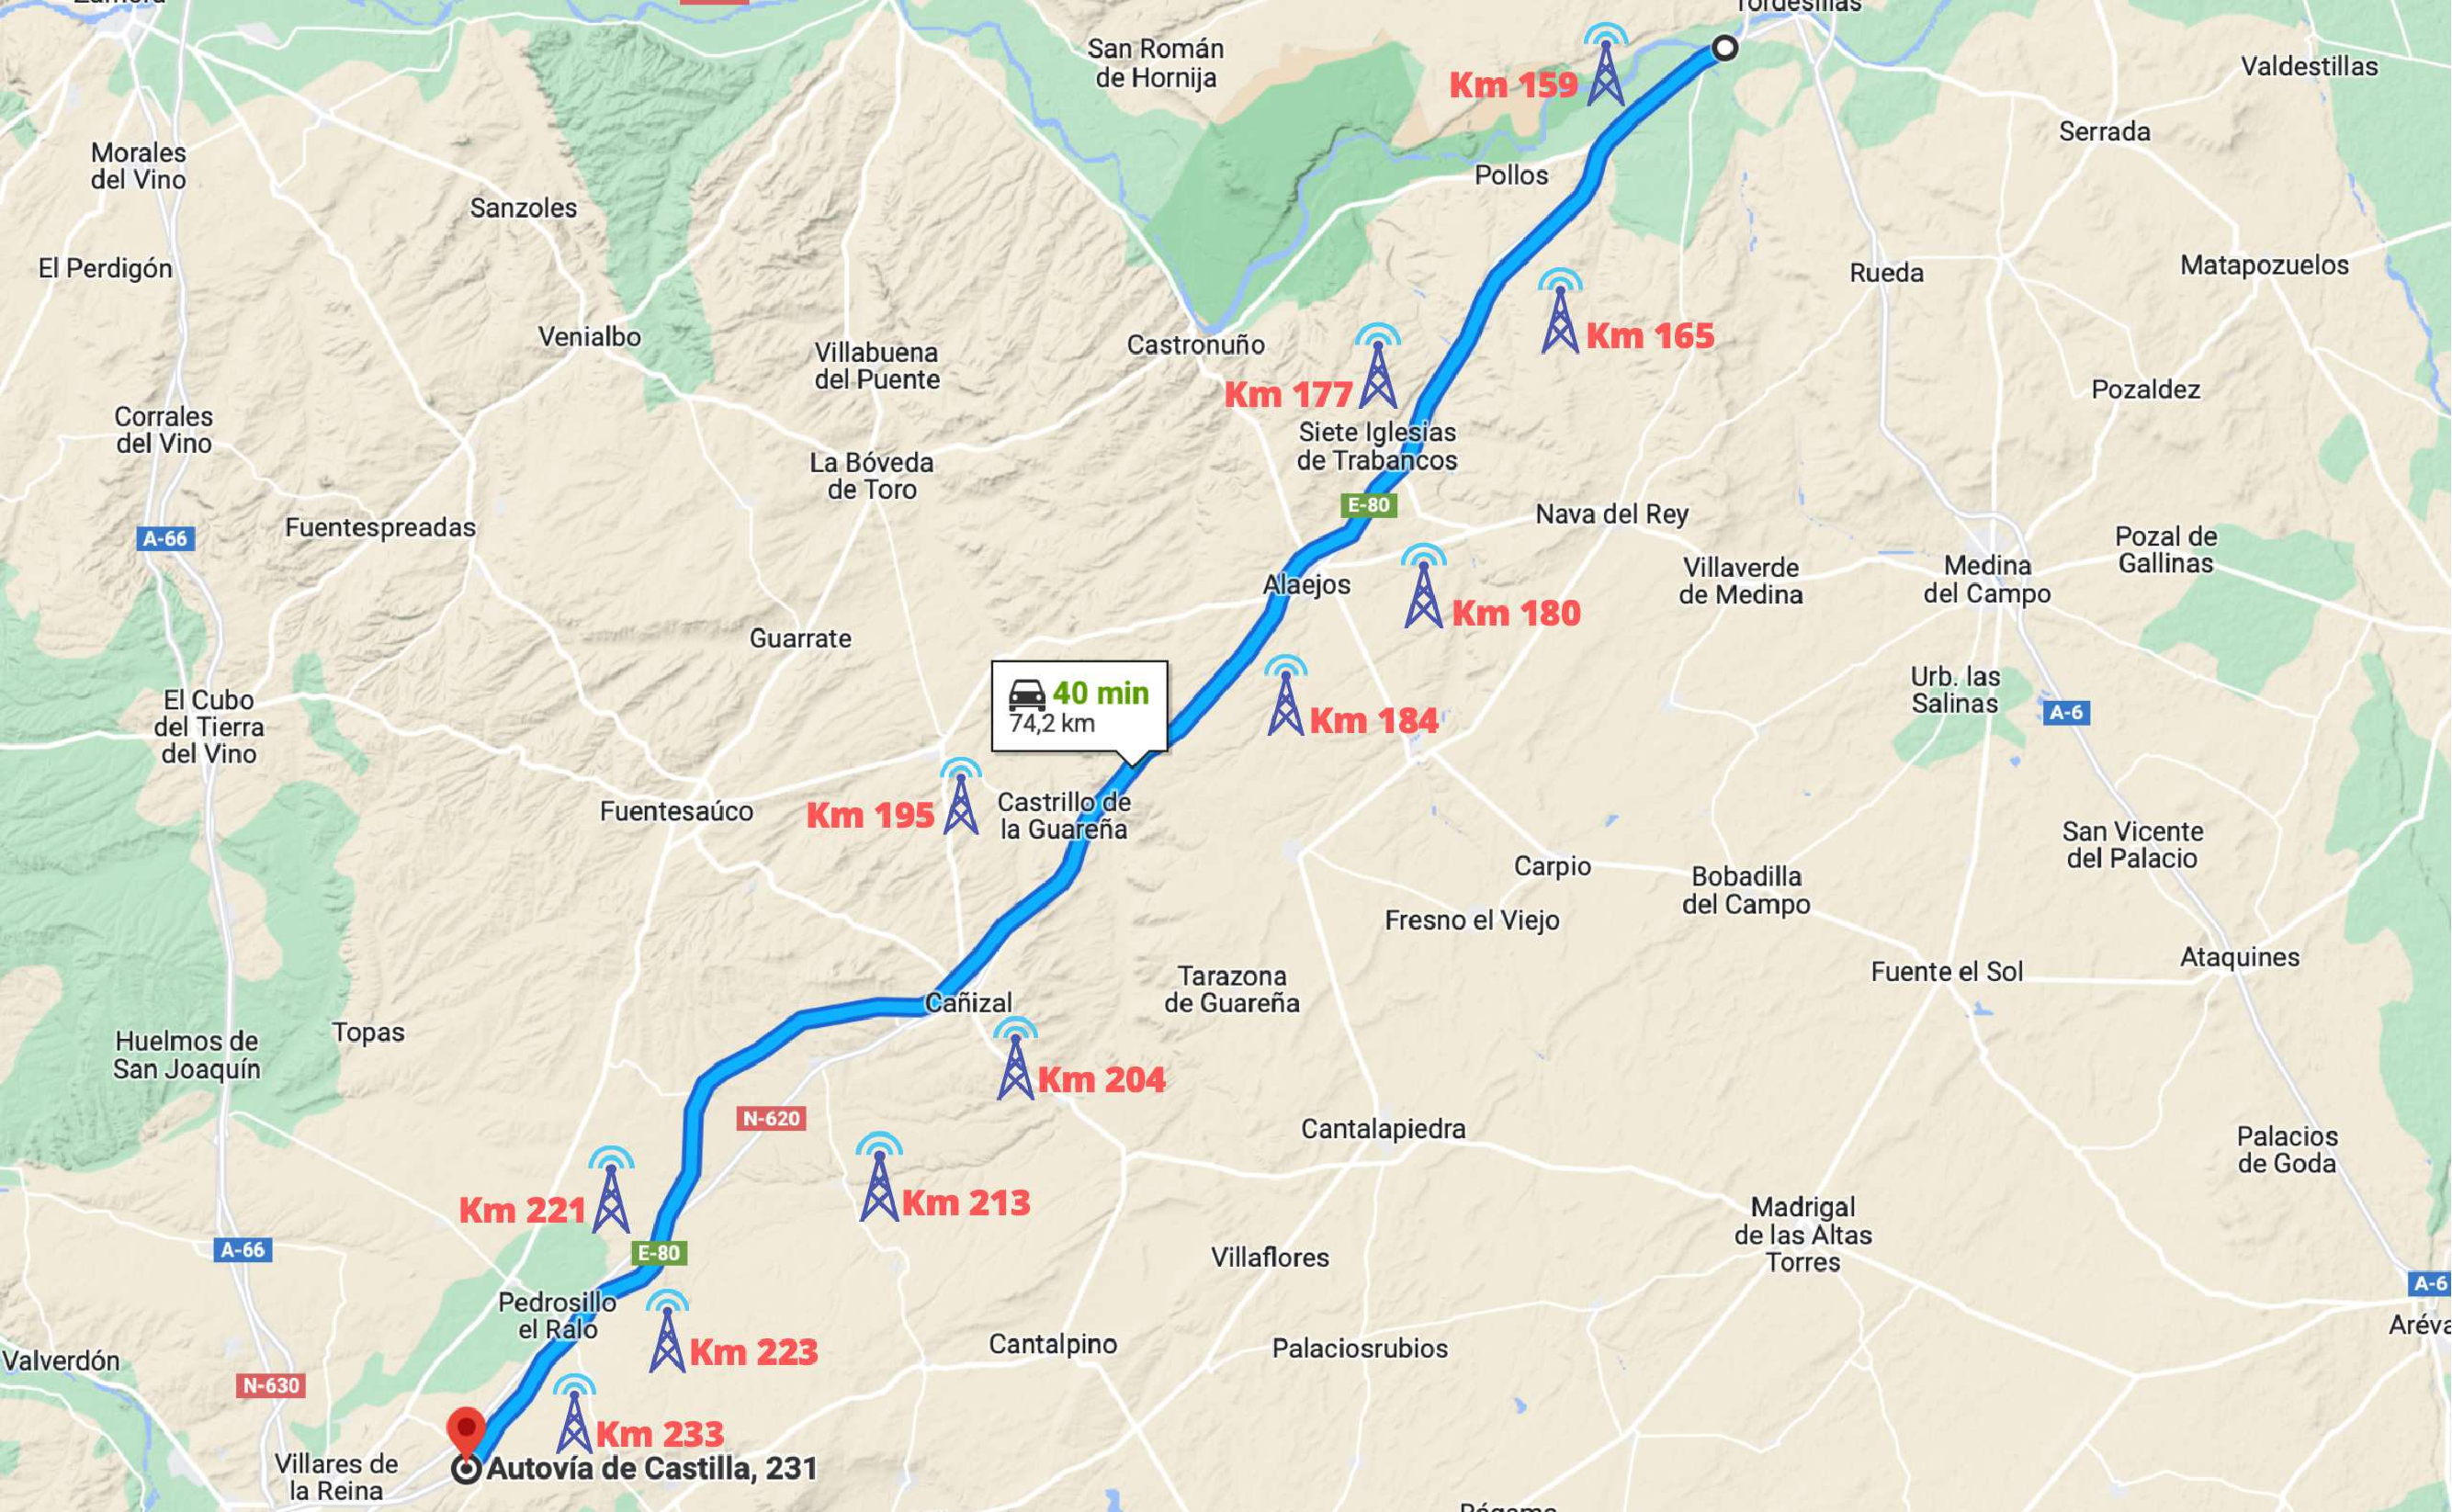
\includegraphics[width=\textwidth]{Imagenes/PlanteamientoInicial/torres_telefonia.pdf}
    \caption{Mapa de la autovía A-62 y las torres de comunicación existentes }
    \label{autovia}
\end{figure}

Queremos que un número elevado de coches pueda hacer uso de dicho servicio de manera ininterrumpida, es decir, se requiere que cada coche tenga capacidad suficiente para enviar el vídeo captado por la cámara durante todo el recorrido. Por ello, es necesario disponer de un ancho de banda de al menos varios Mbps dependiendo de la calidad del vídeo. \\

Prestando este servicio, los vehículos de los usuarios tendrán la capacidad de detectar las señales de tráfico aumentando así la seguridad vial, ya que así los vehículos pueden adaptar su velocidad y comportamiento en la carretera, lo que puede reducir el riesgo de accidentes y mejorar la seguridad vial en general. De igual forma, puede fomentar el cumplimiento de las normativas y regulaciones de tráfico, reduciendo así la cantidad de sanciones, o puede ayudar a optimizar el consumo de combustible y reducir las emisiones de gases contaminantes.\\
